%%%%%%%%%%%%%%%%%%%%%%%%%%%%%%%%%%%%%%%%%%%%%%%%%%%%%%%%%%%
%
%		Relazione del progetto di Sistemi Operativi
%
%				    Nicola Corti - 2011
%
%%%%%%%%%%%%%%%%%%%%%%%%%%%%%%%%%%%%%%%%%%%%%%%%%%%%%%%%%%%
\documentclass[a4paper,10pt]{article} 
\usepackage{graphicx}
\usepackage{vmargin}
\usepackage[italian]{babel} 
\usepackage[latin1]{inputenc}


\setpapersize{A4}
\setmarginsrb{15mm}{10mm}{15mm}{10mm}%
             {0mm}{10mm}{0mm}{10mm}
 
\title{\texttt{cars}: un semplice sistema di car sharing \\ Relazione finale del progetto}
\author{Nicola Corti - 454413 \\Corso di Laurea in Informatica (L-31) - Universit\`a di pisa}
\date{12 Luglio 2011}

 
\begin{document}
\maketitle 
 
\begin{abstract}
Questa relazione ha lo scopo di illustrare i dettagli implementativi del sistema di car sharing \texttt{cars}, nel caso in cui si fosse invece  interessati soltanto alla guida per l'uso si pu\`o consultare la documentazione dell'utente, in allegato al kit d'installazione
\end{abstract}
 
\tableofcontents
 
\section{Il Server - mgcars}

Il server \texttt{mgcars} rappresenta il nucleo di tutto il sistema \texttt{cars}.

Una rappresentazione schematica del server pu\`o essere espressa mediante il diagramma seguente:
\begin{center}
	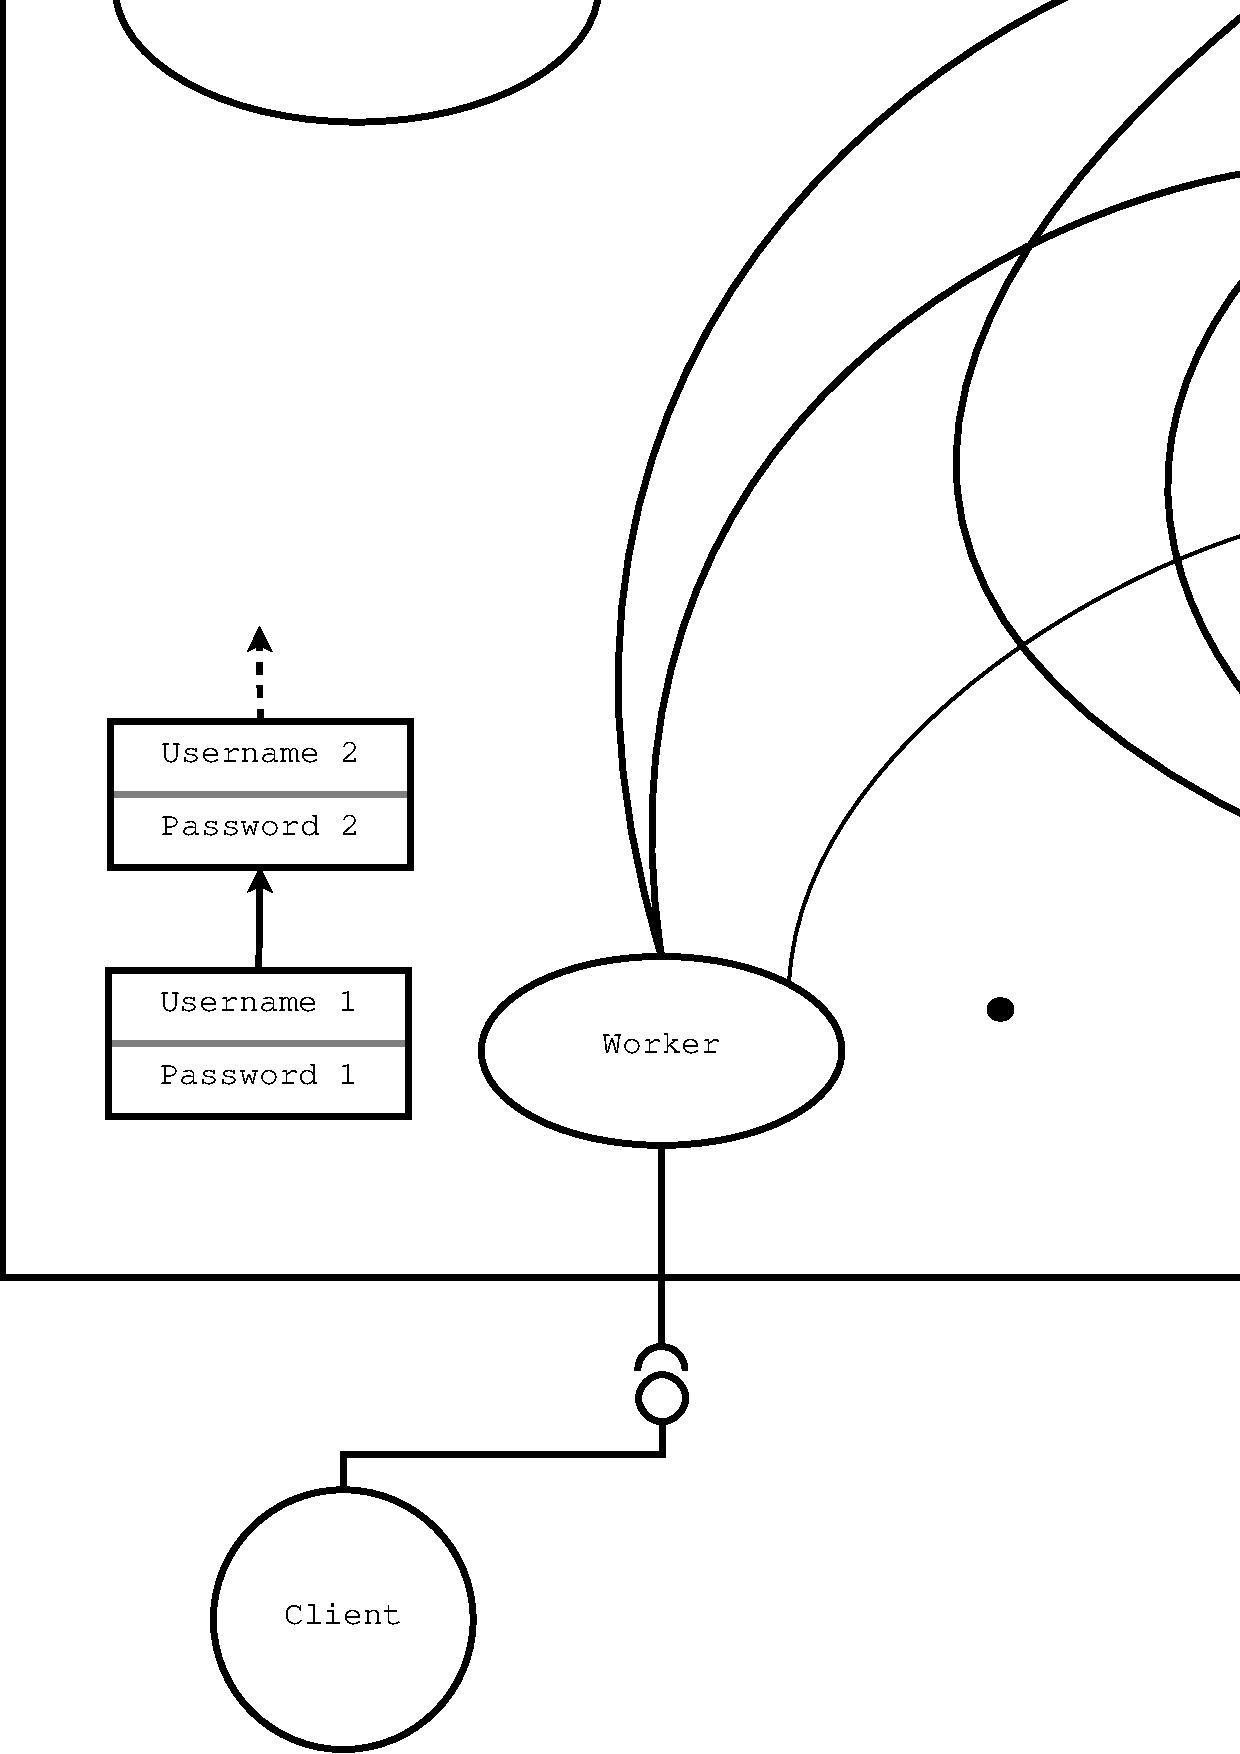
\includegraphics[scale=0.20]{../doc/tex/img/server.png}
\end{center}
Al suo avvio il server esegue in ordine i seguenti passi:

\begin{itemize}
	\item Cerca di caricare in memoria un grafo orientato partendo dai file 
	delle citt\`a e degli archi che sono dati in input.
	\item Cerca di aprire il file di log specificato dalla macro LOG\_FILE\_NAME.
	\item Prova a far partire i thread worker.	
	\item Prova a far partire il thread gestore dei segnali.
	\item Prova a far partire il thread match.
	\item Apre una socket in ascolto all'indirizzo specificato dalla macro SOCKET\_PATH.	
\end{itemize}

Una volta che tutti questi passi sono stati eseguiti correttamente il server \`e pronto per ricevere connessioni in entrata.

Per quanto riguarda i thread si \`e deciso di provare ad avviarli, nel caso non vi fossero sufficienti risorse attendere DELAY secondi e riprovare per MAX\_TRY volte.\footnote{Nel caso comunque che il server non riesca ad avviare dei thread per mancanza di risorse, si prenda in considerazione la possibilit\`a di variare i parametri del server o di cambiare elaboratore.}

\subsection{Il thread main}

Da questo momento in poi il thread main resta in ascolto sulla socket appena aperta di eventuali connessioni e le schedula ad un thread fra quelli presenti nel pool.

Lo scheduling viene effettuato con politica \emph{round robin}, grazie alla funzione findActivateThread, contenente un variabile statica che viene utilizzata per cercare nel pool un thread disponibile a servire un nuovo utente.

Con uno scheduling di questo tipo si \`e certi che il carico di lavoro viene ripartito in modo equo fra gli worker e non sono presenti worker che rimangono dormienti per tutto il tempo dell'esecuzione del server.

Una volta trovato un thread che \`e in attesa lo si attiva e gli si comunica il socket sul quale pu\`o mettersi in attesa di messaggi in entrata.

Nel caso in cui non sia possibile trovare un thread disponibile, si \`e deciso di chiudere il socket relativo al client appena connesso e di non comunicare al client che il server ha raggiunto il suo carico massimo; cos\`i da tentare di sventare attacchi del tipo DoS (l'utente, non essendo a conoscenza del fatto che il server \`e sovraccarico, potrebbe imputare il problema ad altri fattori).

\subsubsection{Il pool di thread}

Si \`e deciso di implementare gli worker mediante un pool di thread la cui dimensione viene stabilita dalla macro POOL\_SIZE.

\`E stata operata questa scelta al fine di conferire maggiore stabilit\`a al server ed una maggiore adattabilit\`a; dato che l'amministratore del server pu\`o definire il numero di thread da utilizzare in funzione dell'infrastruttura a sua disposizione.

Di fatto il pool di thread \`e un vettore di strutture \texttt{worker\_t} cos\`i definite:
\begin{verbatim}
typedef struct worker{
    pthread_t tid;
    int in_sck;
    int out_sck;
    int active;
    pthread_cond_t cond;
    int sentreqs;
} worker_t;
\end{verbatim}

\begin{description}
	\item[tid] Rappresenta il Thread Identifier dello specifico thread, utilizzato per interagire con il singolo thread (invio di segnali, join, etc...).
	\item[in\_sck] Socket in entrata, viene settata dal thread main all'atto dell'attivazione del thread. Quando il thread non \`e attivo vale -1.
	\item[out\_sck] Socket in uscita, viene settata dal singolo worker, nel momento in cui ci si riesce a connettere sul socket specificato dall'utente. Quando il thread non \`e attivo vale -1, a meno che il server non abbia avviato la procedura di spegnimento e il numero delle richieste inviate sia maggiore di 0. In tal caso il thread match, dopo che avr\`a calcolato gli ultimi accopiamenti, invier\`a i dovuti messaggi e chiuder\`a lui stesso i socket in uscita.
	\item[active] Bit che indica se il singolo thread \`e attivo oppure se \`e in attesa di una nuova connessione.
	\item[cond] Variabile di tipo \texttt{pthread\_cond\_t} su cui il thread resta in attesa ed \`e utilizzata per risvegliarlo e per farlo partire.
	\item[sentreqs] Numero di richieste inviate (non necessario ai fini del pool di thread, ma viene utilizzato dal thread match per inviare i messaggi di SHARE\_END).
\end{description}

Tutto il pool viene gestito in mutua esclusione grazie alla variabile \texttt{mux\_pool} di tipo \texttt{pthread\_mutex\_t}, dato che tutti i thread accedono al pool per leggere e per modicare i dati.

\subsection{Il thread worker}

All'avvio ogni thread worker si mette in attesa di essere attivato dal thread main, restando bloccato su \texttt{waitForActivation}.

Una volta attivato attende di ricevere il messaggio di login sul socket indicato nella sua struttura: se il messaggio \`e un messaggio di login valido (come definito dal protocollo di comunicazione) allora ne estrapola i dati necessari per verificare il login.

Se il messaggio non \`e un messaggio di login valido, il thread torna in attesa invocando la funzione \texttt{goingBackToSleep} che lo riporta in stato di attesa. Anche in questo caso si \`e deciso di terminare immediatamente la comunicazione col client, perch\'e probabilmente si tratta di un client che non sta funzionando a dovere, o peggio, di un client manomesso, che potrebbe inficiare la corretta esecuzione del server.

\subsubsection{Autenticazione dell'utente}

Una volta estrapolati i dati dell'utente si passa alla sua autenticazione:
i dati degli utenti vengono salvati in chiaro in una lista linkata di questo tipo:
\begin{verbatim}
typedef struct credential{
    char username[LUSERNAME];
    char password[LUSERNAME];
    int active;
    struct credential *next;
} credential_t;
\end{verbatim}
\begin{description}
	\item[username] Nome utente.
	\item[password] Password (salvata in chiaro\footnote{Si sarebbe potuto salvare l'hash della password pi\`u un eventuale seme e controllare mediante questi ultimi l'identit\'a dell'utente (in un modo similare a quanto avviene nei sistemi UNIX/Linux), ma non era questo l'obiettivo del progetto.}).
	\item[active] Bit che indica se un utente \`e gi\`a loggato presso un worker in questa sessione del server.
	\item[next] Puntatore alla prossima struttura.
\end{description}

Anche questa struttura viene acceduta in mutua esclusione grazie alla variabile \texttt{mux\_pool}.

I possibili esiti della procedura di autenticazione dell'utente \texttt{isAlreadyUser}, possono essere:

\begin{itemize}
	\item \textbf{Esiti positivi}
	\begin{itemize}
		\item Utente non presente: si provvede ad inserire una nuova occorrenza nella lista degli utenti e a settare l'utente come attivo.
		\item Utente non attivo e password corretta: si provvede a settare l'utente come attivo.
	\end{itemize}
	\item \textbf{Esiti negativi}
	\begin{itemize}
		\item Password errata: la password non corrisponde con quella utilizzata nelle precedenti sessioni, si invia perci\`o il messaggio di errore.
		\item Utente gi\`a attivo: l'utente risulta gi\`a loggato presso un altro worker quindi si invia il messaggio di errore.
		\item Utente o Password invalidi: indica che la stringa del login \`e malformata (probabilmente \`e presente un malfunzionamento nel client).
	\end{itemize}
\end{itemize}
Nei casi di esito positivo, si invia il messaggio di conferma e si inizia la sessione di ricezione messaggi con il client. Nei casi di esito negativo il thread torna in fase di attesa.

\subsubsection{Sessione di ricezione messaggi}

Durante la sessione di ricezione messaggi, il worker sta in attesa sulla socket in entrata di messaggi da parte del client.

La correttezza sintattica dei messaggi viene controllata dal client (in modo da non far fare ulteriori elaborazioni al server) per cui si assume che i messaggi in arrivo dal client siano corretti. Dobbiamo invece verificare che le localit\`a inviate siano presenti nella mappa caricata sul server.

Ci\`o \`e controllato dalla procedura \texttt{checkValidMessage}, che in base al valore ritornato permette di capire se si pu\'o accettare l'offerta/richiesta o meno (nome della citt\`a di partenza/arrivo non presente, troppo lungo, problema con il numero dei posti, etc...).

Nel caso in cui l'esito sia positivo si provvede ad accodare la richiesta o l'offerta nella rispettiva coda (e ad incrementare il numero delle richieste ricevute, se necessario).

La sessione termina se cade la connessione, se il client invia il messaggio di exit oppure se \`e stato ricevuto il segnale di terminazione; in tali casi si provvede a sloggare l'utente e a tornare in modalit\`a di attesa.

\subsection{Il thread match}

Il thread match sta costantemente in attesa su una \texttt{sigtimedwait} di un segnale SIGUSR1. Nel caso in cui il segnale non arrivi entro SEC\_TIMER secondi e NSEC\_TIMER nanosecondi, il thread match parte ugualmente ed inizia a cercare degli accoppiamenti.

Le richieste e le offerte pervengono al match mediante due code distinte. Si \`e deciso di utilizzare tale struttura dati per servire le richieste con una politica \textit{FIFO} (le prime richieste che sono pervenute sono le prime che saranno servite).

Le code sono implementate mediante delle liste linkate, dove gli inserimenti vengono effettuati in coda, e le estrazioni in testa, con delle strutture di questo tipo:

\begin{verbatim}
typedef struct reqoff{
    int type;
    char user[LUSERNAME];
    char depart[LLABEL];
    char arriv[LLABEL];
    int place;
    int share_fd;
    char *path
    struct reqoff *next;
} reqoff_t;
\end{verbatim}
\begin{description}
	\item[type] indica se si tratta di un'offerta o di una richiesta.
	\item[user] utente che ha inviato la richiesta/offerta.
	\item[depart] localit\`a di partenza.
	\item[arriv] localit\`a di arrivo.
	\item[place] numero dei posti, nel caso delle offerte.
	\item[share\_fd] indice della socket dove si deve inviare la risposta (nel caso delle richieste).
	\item[next] puntatore al prossimo elemento della coda.
	\item[path] puntatore ad una stringa che indica il cammino minimo fra la localit\`a di partenza e la localit\`a di arrivo.
\end{description}

La stringa path rappresenta il cammino minimo fra le due localit\`a ed \`e generata dai worker, nel momento in cui inseriscono nelle code una nuova richiesta/offerta, cos\'i da non rendere pi\'u oneroso il carico del match.

Le due code vengono gestite in mutua esclusione mediante due variabili \texttt{pthread\_mutex\_t}. Si \`e deciso di gestirle con due variabili distinte in modo che l'aggiunta di una richiesta e di un'offerta possa essere eseguita in modo concorrente.

\subsubsection{La ricerca di accoppiamenti}

Una volta avviata la fase di match, il thread acquisisce la mutua esclusione sulle due code e sul pool di thread\footnote{In questo modo gli worker e il main restano bloccati in attesa della terminazione della fase di match; se infatti si accettassero ulteriori richieste/offerte il thread match potrebbe trovarsi a lavorare in uno stato inconsistente.}.

Quindi il thread inizia a cercare degli accoppiamenti per ogni elemento della coda richieste, invocando la funzione \texttt{findAssociation}. Tale funzione utilizza a sua volta la funzione \texttt{findRec} che indica se esiste o meno un possibile percorso che riesca a soddisfare la richiesta\footnote{Tale esito \`e rappresentato dai valori TRUE o FALSE, che sono di fatto delle macro con valori rispettivamente 1 e 0, settate al fine di rendere pi\`u leggibile il codice}.

La funzione \texttt{findRec} \`e una funzione ricorsiva che opera sulle stringhe del path e cerca di costruire un percorso per soddisfare la richiesta. Nel caso in cui riesca a costruirlo lo salva in una lista di tipo \texttt{assoc\_t}.
\begin{verbatim}
typedef struct assoc{
    int city_found;
    int begin_from;
    reqoff_t *found_off;
    struct assoc *next;
} assoc_t;
\end{verbatim}

\begin{description}
	\item[city\_found] rappresenta il numero di citt\`a che sono state trovate che corrispondono in quella offerta.
	\item[begin\_from] rappresenta il numero ci citt\`a da cui parte il percorso trovato (vedi esempio).
	\item[found\_off] rappresenta il puntatore all'offerta che corrisponde a questa parte di percorso.
	\item[next] puntatore al prossimo passo nel percorso.
\end{description}

\begin{small}
\textbf{Esempio 1:} Se l'offerta relativa alla prima parte del percorso ha il seguente path: \texttt{PISA\$LUCCA\$ALTOPASCIO\$PISTOIA} e i valori delle variabili sono \texttt{city\_found = 2} e \texttt{begin\_from = 1} allora il percorso effettuato in questo passo sar\`a \texttt{LUCCA\$ALTOPASCIO}.
\end{small}

\medskip 

La procedura fa uso delle funzioni definite nell'header \texttt{match.h} e implementate nel sorgente \texttt{match.c}

Se la ricerca del percorso ha avuto esito positivo, si provvede a scrivere sul file di log gli accoppiamenti, ad inviare i messaggi di SHARE e ad aggiornare la lista delle offerte.

\subparagraph{Implementazione alternativa: il vettore dei precedenti}
\begin{small}
Si sarebbe potuto implementare la ricerca utilizzando il vettore dei precedenti restituito dall'algoritmo di \textit{Dijkstra}, ma si \`e deciso di utilizzare la ricerca su stringhe, malgrado la maggiore difficolt\`a, perch\'e i percorsi generati tendono ad avere la prima tappa pi\`u lunga possibile.

Una ricerca sul vettore dei precedenti avrebbe generato percorsi con l'ultima tappa pi\`u lunga, essendo una ricerca effettuata all'indietro.

Generando percorsi con la prime tappe pi\`u lunghe si cerca di ``aiutare'' gli utenti facendoli avvicinare il pi\`u possibile alla loro destinazione, in modo che se gli offerenti che avrebbero dovuto accompagnarli a destinazione dovessero venire meno all'impegno stabilito, la distanza per raggiungere la destinazione sia la minore possibile (favorendo l'uso di mezzi di trasporto pubblico).
\end{small}

\subsubsection{L'aggiornamento delle offerte}

Se la macro UPDATE\_OFFER risulta definita, il match scomporr\`a ogni richiesta che compone una parte del percorso in modo da poter sfruttare a pieno tutti i posti disponibili di ogni offerta. Un esempio chiarir\`a meglio il concetto:

\begin{small}
\textbf{Esempio 2:} se l'offerta relativa avesse avuto 4 posti disponibili, sarebbe stata scomposta in altre 3 offerte, una con path \texttt{PISA\$LUCCA\$ALTOPASCIO\$PISTOIA} e 3 posti, e altre 2 offerte da 1 posto relative a \texttt{PISA\$LUCCA} e \texttt{ALTOPASCIO\$PISTOIA}.
\end{small}


\subsubsection{Fase finale}
Dopo aver elaborato tutte le richieste, il thread match invia il messaggio di SHARE\_END a tutti i client che hanno inviato almeno una richiesta (tale informazione la pu\`o ricavare dai dati nella struttura del pool di thread).

La lista delle richieste pendenti viene completamente liberata.

Se risulta settata la macro FREE\_OFF\_LIST la lista delle offerte viene liberata, altrimenti le richieste vengono  mantenute\footnote{ATTENZIONE: se si decide di scompattare l'offerta e di non liberare la lista delle offerte si potrebbero avere dei rallentamenti sul server nel lungo termine, dato che le offerte risultano parecchio frammentate; ci\`o potrebbe rendere pi\`u lungo il processo di ricerca di un percorso (rimarrebbero infatti tanti piccole offerte da un posto con path molto brevi).}.

\subsection{Il thread signal\_handler e la terminazione del server}

Il thread gestore dei segnali resta costantemente in attesa (mediante una \texttt{sigwait}) di un segnale in arrivo. A questo thread vengono indirizzati tutti i messaggi in arrivo al processo, tranne il segnale SIGUSR1 che viene recapitato al thread match.

Per i segnali di errore di sistema (SIGSEGV, SIGILL, etc...) \`e stato installato un gestore che gestisce la terminazione immediate e visualizza un messaggio di errore critico su \textit{standard error}\footnote{In modo da evitare la visualizzazione di messaggi sgradevoli su terminale (quali ad esempio Segmentation Fault, etc...)}.

Il segnale di SIGPIPE viene ignorato per non far terminare il processo.

I segnali di SIGINT e SIGTERM provocano invece l'inizio della fase di terminazione del processo, il thread signal\_handler esegue allora in ordine i seguenti passi:

\begin{enumerate}
	\item Setta ad 1 la variabile globale \texttt{received\_signal} che indica che sta iniziando la procedura di spegnimento del server.
	\item Risveglia tutti gli worker e gli invia un segnale SIGUSR2.
	\item Setta a 2 la variabile globale \texttt{received\_signal} ad indicare che gli worker sono terminati e il match pu\`o eseguire per l'ultima volta la procedura di ricerca delle associazioni.
	\item Invia il segnale di SIGUSR1 al thread match per sbloccarlo.
	\item Attende la terminazione del thread match.
	\item Chiude i socket che eventualmente sono rimasti aperti dato che il thread match li ha utilizzati per inviare gli ultimi messaggio di SHARE e di SHARE\_END.
	\item Invia un segnale di SIGUSR2 al thread main per sbloccarlo nel caso fosse rimasto bloccato su una accept.
	\item Il thread signal\_handler termina.
\end{enumerate}

Nel frattempo il thread main si \`e messo in attesa della terminazione del thread signal\_handler, appena \`e terminato esegue le ultime operazioni di pulizia del sistema:
\begin{itemize}
	\item Libera la memoria allocata dalla lista degli utenti.
	\item Chiude il \emph{file descriptor} relativo al socket sul quale il main accettava le connessioni entranti.
	\item Rimuove il file che rappresenta la socket da disco.
	\item Libera la memoria allocata dal grafo orientato.
	\item Chiude il \textit{file descriptor} relativo al file di log.
\end{itemize}

Se tutti questi passi vengono eseguiti correttamente, anche il thread main termina e il processo ritorna con 0 come valore d'uscita\footnote{In questo modo il programma risulta conforme alle convenzioni bash (dove 0 indica uno stato d'uscita corretto) e pu\`o essere utilizzato all'interno di script bash senza problemi.}. In tutti gli altri casi il processo ritorna con uno stato diverso da 0.

\section{Il Client - docars}

Il client \texttt{docars} rappresenta l'interfaccia nei confronti dell'utente del sistema \texttt{cars}.

Il client consta di due thread: il thread \texttt{main} a cui \`e demandata la relazione diretta con l'utente, l'accettazione di messaggi, la loro verifica e l'invio al server, ed il thread \texttt{listener} che si occupa di riceve i messaggi in ingresso da parte del server.

Il client viene avviato avendo come unico parametro l'username dell'utente che desidera collegarsi al sistema. Il client provvede quindi a chiedere all'utente la sua password e a generare un nome univoco per la sua socket; si \`e deciso di generare il nome della socket concatenando il nome utente al PID del processo, cos\`i che il nome della socket sia univoco.\footnote{Tale assunzione non \`e totalmente vera, potrebbero infatti crearsi interferenze se rimanesse sul file system un file relativo ad una socket di un client (a causa per esempio di un suo arresto improvviso) e lo stesso utente riavviase il client ottenendo lo stesso PID precedente. Questo evento ha comunque una possibilit\`a comunque molto ridotta di verifirsi, tale da poterci permettere di definire questo nome di socket cos\`i generato, univoco.}

Il client cerca dunque di collegarsi al server e gli invia i dati relativi all'utente. Successivamente attende una connessione in ingresso sul socket il cui nome \`e stato generato precedentemente. Cerca quindi di leggere l'esito della connesione al server: se l'esito \`e positivo l'utente \`e riuscito ad autenticarsi correttamente, inizia la sessione interattiva (gestita dal thread \texttt{main}) e la ricezione dei messaggi dal server (gestita dal thread \texttt{listener}) , altrimenti l'esecuzione del client termina visualizzando il messaggio di errore inviato dal server.

\subsection{La sessione interattiva}

Durante la sessione interattiva il thread \texttt{main} presenta il prompt (definito dalla macro PROMPT) e si mette in attesa di dati su \textit{standard input} mediante la funzione di libreria \texttt{fgets}\footnote{Nel caso in cui il messaggio si pi\`u lungo di BUFF\_SIZE si segnala un errore e si provvede a rimuovere i caratteri in eccesso da \textit{standard input}.}; provvede dunque a verificarne la sua correttezza mediante la funzione \texttt{messageParser} e a preparare eventualmente un messaggio da inviare al server.

Si \`e deciso di verificare la correttezza sintattica delle richieste/offerte nel client, come gi\`a detto in precedenza, per non sovraccaricare inutilmente di lavoro il server.

Se si tratta di un messaggio valido di richiesta o di offerta, si provvede ad inviarlo al server e ci si mette in attesa dell'esito dal server.

Se si tratta di un messaggio di HELP o di un messaggio sintatticamente scorretto, si provvede a visualizzare dei messaggi informativi a schermo e si torna in attesa di un input dall'utente.

Se si tratta di un messaggio di EXIT oppure l'utente ha inviato un EOF, si invia un messaggio di EXIT al server e si conclude la sessione interattiva. Dopo di che, se sono state inviate richieste di recente, si attendono eventuali messaggi di SHARE\_END da parte del server, altrimenti il client termina la sua esecuzione.

\subsection{Il thread listener}

Il thread \texttt{listener} ha come compito primario quello di restare in attesa di messaggi in arrivo dal server. I messaggi che possono arrivare dal server sono di 2 tipi:

\begin{itemize}
	\item Messaggi di OK e di NO, che vengono ricevuti in seguito a messaggi di richieste od offerte inviate dal client stesso. Questi messaggi vengono considerati di tipo \emph{sincrono}, dato che possono essere ricevuti soltanto in seguito all'invio di un messaggio. Inoltre senza aver ricevuto un messaggio di questo genere, il thread \texttt{main} non pu\`o inviare ulteriori messaggi.
	\item Messaggi di SHARE e di SHARE\_END, che possono essere ricevuti in un qualsiasi momento, purch\'e in un passato prossimo sia stata inviata una richiesta dal client e tale richiesta sia stato seguita da un messaggio di OK. Tali messaggi vengono considerati \textit{asincroni} dato che possono essere ricevuti in ogni momento.
\end{itemize}

\subsubsection{Mutua esclusione fra i due thread}

Per gestire una corretta interazione fra client e server sono state definite alcuni flag globali e alcune variabili per gestire la mutua esclusione:

\begin{description}
	\item[\texttt{message\_sem}] Se vale 0, vuol dire che il \texttt{main} pu\`o inviare un messaggio al server. Una volta che il messaggio \`e stato inviato, tale flag viene settato a 1. Verr\`a successivamente risettato a 0 dal \texttt{listener} nel momento in cui si riceve un messaggio di OK o di NO. Per gestire la mutua esclusione di questa variabile vengono utilizzate la variabili \texttt{mux} e \texttt{cond}, rispettivamente di tipo \texttt{pthread\_mutex\_t} e \texttt{pthread\_cond\_t}; il thread \texttt{main} si mette infatti in attesa su \texttt{cond} che il flag diventi 1 per potere inviare un nuovo messaggio.

	\item[\texttt{sharend\_sem}] Il suo valore di default \`e 0, viene settato a 1 da \texttt{main} se si \`e inviata un'offerta, e successivamente viene settato a 2 da \texttt{listener} se la risposta a tale richiesta \`e stata OK. Serve per capire se si deve attendere un messaggio di SHARE\_END o meno da parte del server; una volta ricevuto il messaggio di SHARE\_END tale flag viene resettato a 0. Il tipo di questa variabile \`e \texttt{volatile sig\_atomic\_t} in modo da poter trascurare l'utilizzo di variabili ausiliarie (\texttt{mutex}) per la gestione della mutua esclusione.
	
	\item[\texttt{end\_prompt}] Il suo valore di defautl \`e 0, vale 1 se \`e terminata la sessione interattiva del \texttt{main}. Ci\`o serve a segnalare al thread \texttt{listener} che, se non vi sono pi\`u SHARE\_END da ricevere, pu\`o terminare la sua esecuzione, altrimenti si mette in attesa dell'ultimo SHARE\_END e successivamente termina la sua esecuzione. Anche questo flag risulta del tipo \texttt{volatile sig\_atomic\_t} per il motivo sopra indicato.
	
\end{description}

\subsection{Terminazione del client}

Per quanto riguarda la terminazione del client, si \`e utilizzato il meccanismo dell'\emph{interrupted system call}.

Per i segnali di errore di sistema (SIGSEGV, SIGILL, etc...), proprio come \`e stato fatto nel server, \`e stato installato un gestore che gestisce la terminazione immediata e visualizza un messaggio di errore critico su \textit{standard error}.

Il segnale di SIGPIPE viene ignorato per non far terminare il processo.

Per i segnali di SIGINT e SIGTERM \`e stato installato un gestore che setta ad 1 la variabile \texttt{received\_signal} e invia il segnale SIGUSR1 al processo.
I segnali SIGINT e SIGTERM possono essere ricevuti soltanto dal thread \texttt{main}, che nel caso in cui fosse bloccato su una \textit{system call} bloccante, risulta sbloccato; lo stesso discorso vale per il segnale SIGUSR1 rispettivamente al thread \texttt{listner}.

Il thread \texttt{main} si mette dunque in attesa di raccogliere il valore di ritorno del thread \texttt{listener} e, successivamente, termina l'esecuzione del client.

\section{Parametri d'esecuzione}

Mediante il file \texttt{settings.h} \`e possibile impostare i parametri d'esecuzione del sistema\footnote{Si noti che il file contiene la direttiva \texttt{\#include <stdlib.h>} dato che altrimenti il compilatore \texttt{gcc} genera un warning, non riuscendo a trovare del codice sorgente C}.

I commenti al file indicano il significato di ogni parametro, i valori consigliati e il possibile impatto sulle prestazioni che pu\`o avere l'incremento o il decremento di un determinato parametro.

Se ne consiglia un'attenta lettura prima di installare il server/client.

Fra i valori che \`e possibile personalizzare vi \`e la possibilit\`a di cambiare il nome della socket del server, il numero di thread, il tempo di attesa del thread match; vi \`e la possibilit\`a di impostare o meno l'aggiornamento delle offerte (come descritto nel paragrafo relativo al thread match).

Fra le varie cose e' inoltre possibile settare la macro VERBOSE, che stampa a video ulteriori messaggi informativi, oltre a quelli gi\`a visualizzati, che possono essere d'aiuto nel comprendere cosa sta facendo il server e/o il client.

I parametri con cui \`e stato compilato il server vengono visualizzati al suo avvio, cos\`i da esplicitare l'ambiente di esecuzione del server.

Inoltre sono disponibili due file: \texttt{settings\_low.h} e \texttt{settings\_high.h} che contengono alcuni parametri predefiniti per l'esecuzione rispettivamente su una macchina di bassa potenza e su una macchina di potenza elevata.

Si ricorda che non \`e sufficiente modificare i valori e riavviare il server/client, ma \`e necessario ricompilarli (\textbf{NOTA BENE:} vanno ricompilati entrambi, altrimenti si pu\`o incorrere in malfunzionamenti del sistema).

\section{Lo script bash - carstat}

Lo script \texttt{carstat} \`e uno script bash che elabora le informazioni del file di log emesso dal server.

Il \textit{parsing} delle opzioni viene effettuato con l'utility \texttt{getopts}.

Per quanto riguarda la sua implementazione si \`e deciso di utilizzare un approccio di tipo iterativo, utilizzando tre array, che contengano rispettivamente i nomi degli utenti, il numero delle offerte effettuate e il numero delle richieste effettuate.

I commenti presenti nel codice risultato sufficienti a comprendere la logica applicativa dello script.

\subsection{I valori di uscita}

Sono stati definiti i seguenti valori di uscita, in modo da comprendere se l'elaborazione \`e andata o meno a buon fine, ed eventualmente la causa dell'errore:\\

\begin{tabular}{|c|l|}
\hline
0 & Esecuzione terminata correttamente.\\
\hline
2 - (ENOENT) & Il file non esiste o non \`e un file regolare.\\
\hline
7 - (E2BIG) & Un parametro \`e stato inserito troppe volte.\\
\hline
13 - (EACCESS) & Non si hanno i diritti di lettura di un file.\\
\hline
22 - (EINVAL) & I parametri inseriti non sono corretti.\\
\hline
\end{tabular}

\subsection{Opzioni aggiuntive}

Inoltre sono state aggiunte delle opzioni aggiuntive, oltre a quelle richieste nelle specifiche del progetto:
\begin{description}
	\item[-d] Visualizza le informazioni separate per ogni file che viene passato in input.
	\item[-h] Visualizza un breve messaggio di aiuto sui possibili parametri.
	\item[-v] Visualizza il numero di versione dello script.
\end{description}

Le ultime due opzioni sono state inserite al fine di rendere lo script pi\`u omogeneo con gli applicativi tipici del mondo UNIX/Linux.

\section{La libreria \texttt{dgraph}}

La libreria \texttt{dgraph} \`e stata sviluppata inizialmente con un approccio errato, utilizzando interamente programmazione strutturata in senso stretto.

Tale approccio ha reso molto pi\`u complesso il codice di tale libreria, che si distaccava molto da quelli che sono gli stili di programmazione tipici del linguaggio C, rendendone cos\`i difficile la comprensione. Si \`e dunque deciso di cercare di ``destrutturare'' il codice sorgente per quanto riguarda la parte della verifica dei parametri.

Risulta invece ancora da correggere tutta la parte relativa all'elaborazione.

\subsection{Scelte implementative}

La libreria risulta interamente \textit{thread safe}, visto che sono state utilizzate funzioni solamente \textit{thread safe}. In particolar modo si \`e utilizzata la funzione \texttt{strtok\_r} che \`e una versione rientrante e \textit{thread safe} della funzione \texttt{strtok}.

Per quanto riguarda l'algoritmo di \textit{Dijkstra}, si \`e deciso di implementare la coda di priorit\`a tramite un \textit{heap} (ad esso sono dedicati i file \texttt{heap.c} e \texttt{heap.h}). Tale struttura offre infatti la possibilit\`a di eseguire operazioni di estrazione e di inserzione in tempo logaritmico, favorendo dunque la velocit\`a di ricerca.

\subsection{Utilizzo delle espressioni regolari}

La verifica della correttezza delle stringhe viene effettuata tramite le funzioni definite nell'header file \texttt{stringparser.h}

Per la verifica della correttezza di un possibile arco \`e stato implementato un metodo alternativo che permette di utilizzare le \textit{espressioni regolari} invece che le operazioni su stringhe.

Per attivare questa modalit\`a \`e sufficiente definire la macro REG\_EXPR\_MODE nel suddetto header.

Tale modalit\`a \`e stata comunque introdotta solamente a scopo didattico, dato che rende molto pi\`u onerosa l'elaborazione e se ne sconsiglia l'utilizzo. In particolar modo introduce un notevole ritardo nell'avvio del server\footnote{Precisamente nel momento in cui viene verificata la correttezza del file \texttt{arc\_file}}.

Per generare la libreria \texttt{libcars} utilizzando questo metodo \`e possibile utilizzare il target \texttt{lib1-regexpr}

\section{Stili di programmazione}

Si \`e cercato di utilizzare uno stile di programmazione che si avvicinasse il pi\`u possibile a quello che \`e lo stile dei software di sistema UNIX.

Le operazioni di acquisizione e di rilascio della mutua esclusione sono state incapsulate all'interno di specifiche funzioni (con nomi spesso autoesplicativi), in modo da evitare errori durante la scrittura del codice, e rendere pi\`u agevole la comprensione per un estraneo.

Per quanto riguarda la gestione degli errori, \`e stato definito un header file comune che contiene le macro condivise da entrambi i sorgenti, il file \texttt{commons.h}.

\`E stato infine utilizzato \texttt{valgrind}, uno strumento di verifica del software che ha reso possibile la riduzione al minimo degli errori generati e della memoria allocata e non liberata.

\section{Requisiti Minimi}

Per l'installazione del sistema \`e necessario disporre dei seguenti strumenti:
\begin{itemize}
	\item Un compilatore C (consigliato \texttt{gcc}).
	\item La libreria standard C (consigliato \texttt{lic6-dev}).
	\item Lo strumento di guida alla compilazione \texttt{make}.
\end{itemize}

Il sistema \`e stato testato su alcune macchine sulle quali  installato Ubuntu 11.04 (Natty Narwal) con l'ultima versione del kernel Linux (2.6.38) ed \`e risultato funzionante senza alcuna anomalia.

Il sistema \`e stato inoltre testato sulla macchina \texttt{olivia.cli.di.unipi.it} ed \`e risultato funzionante.

\textbf{Attenzione:} l'esito di \texttt{test31} \texttt{test32} e \texttt{test33} pu\`o variare in base alla dimensione del pool di thread (macro POOL\_SIZE).

\section{Installazione del sistema}

Per installare il sistema \`e possibile utilizzare alcuni target del makefile, creati appositamente per questo scopo:

\begin{description}
	\item[install-client] Ripulisce l'ambiente, ricompila le librerie e installa il client.
	\item[install-server] Ripulisce l'ambiente, ricompila le librerie e installa il server.
	\item[install] Ripulisce l'ambiente, ricompila le librerie e installa sia il server che il client.
\end{description}

Tutti questi target sono corredati da stampe a video che indicano all'utente i passi dell'installazione.

\section{\texttt{stress} - uno script per valutare le prestazioni}

\`E stato scritto un breve script \texttt{bash} che permette di portare il pool di thread al massimo del suo carico, cos\`i da poter valutare le condizioni del sistema in una fase di carico elevato (cos\`i da potersi poi regolare per impostare la dimensione del pool).

Lo script si invoca facilmente con il comando

\begin{center}
	\texttt{./stress.sh <num client> <sec>}
\end{center}

Lo script provvede dunque ad invocare \texttt{num client} distinti ogni \texttt{sec} secondi.

I client vengono generati con nomi differenti\footnote{Viene utilizzato un numero progressivo}, cos\`i che i client non vengano rifiutati per password invalida.

\section{Nota sull'uso dei segnali}

Per inviare il segnale di SIGUSR1 al server \`e possibile utilizzare l'utility \texttt{kill}\footnote{Generalmente presente in tutti i sistemi UNIX/Linux} con la seguente sintassi:
\begin{center}
	\texttt{kill -USR1 <pid>}
\end{center}
Dove \texttt{pid} rappresenta il \textit{process identifier} del processo del server che pu\`o essere ricavato con l'utility \texttt{ps}.

Per inviare il segnale di terminazione si pu\`o utilizzare la combinazione di tasti \texttt{Ctrl-C} se ci si trova nella shell dove \`e stato avviato il processo oppure usare l'utility sopra citata con parametro -INT o -TERM

Nel caso in cui il sistema risulti bloccato utilizzare l'utility sopra citata con parametro -KILL. Cercare di utilizzare il meno possibile questa soluzione, dato che potrebbe lasciare il sistema in uno stato inconsistente.

\textbf{ATTENZIONE:} non inviare assolutamente i segnali SIGUSR2 al server e SIGUSR1 al client. Essi sono utilizzati per gestire la procedura di terminazione dell'applicativo. Una loro ricezione inaspettata potrebbe portare il sistema in stato di blocco.

\section{Bug Noti}

Segue una lista di alcuni bug noti di cui non si \`e riusciti a trovare una soluzione:
\begin{itemize}
	\item Il sistema \`e risultato non funzionante su una vecchia versione di Ubuntu. La compilazione terminava correttamente, ma il client dava un \textit{Segmentation fault} nel momento in cui si invocava la funzione \texttt{sendMessage}. Tale problema sembra essere derivato da un scrittura in una locazione di memoria illecita (\texttt{comsock.c: 207}). 
	Il problema \`e comunque stato risolto con un aggiornamento delle librerie e del compilatore.
	
	Purtroppo non si \`e riusciti a comprendere la causa di questo problema, che comunque non si \`e manifestato su altre macchine.
\end{itemize}

\section{Possibili miglioramenti}

Segue una lista dei possibili miglioramenti che potrebbero essere apportati in futuro, al fine di migliorare il software e di estendere le sue capacit\`a.

\begin{itemize}
	\item Introdurre il supporto per le socket \texttt{AF\_INET} in modo da poter rendere utilizzabile il software anche sulla rete
	\item Introdurre la possibilit\`a di loggarsi al server come \texttt{root} e di poter sottoporre richieste sullo stato attuale del server (ad esempio: stato del pool di thread, stato delle code delle richieste offerte, lista degli utenti loggati, etc...).
	\item Introdurre la possibilit\`a di poter modificare il grafo durante l'esecuzione del server, sempre mediante un accesso privilegiato.
	\item Introdurre una gestione avanzata delle offerte, in modo che si possa comunicare agli utenti che hanno avanzato un'offerta, un elenco delle persone che deve caricare/scaricare ad ogni tappa del percorso.
\end{itemize}

\section{Documentazione allegata}

In allegato al codice sorgente \`e disponibile la documentazione nelle seguenti forme:
\begin{itemize}
	\item Il presente documento, di cui sono disponibili il PDF e i sorgenti \LaTeX\
	\begin{itemize}
		\item Per compilare il \LaTeX\ di questa relazione e per visualizzarne il PDF eseguire il target \texttt{relazione.pdf} (necessari i software \texttt{pdflatex} e \texttt{evince} per compilazione e visualizzazione).
		\item Per compilare il \LaTeX\ di questa relazione e per visualizzarne il PS eseguire il target \texttt{relazione.ps} (necessari i software \texttt{latex} e \texttt{dvips} ed \texttt{evince}).
	\end{itemize}
	\item Le manpages del server, del client e dello script, nella cartella \texttt{doc/man/}
	\begin{itemize}
		\item Per visualizzare le manpages eseguire il target \texttt{man-<software>}, ad esempio \texttt{man-docars} per visualizzare il man di \texttt{docars}.
		\item Per visualizzare il PS delle manpage eseguire il target \texttt{man-<software>-ps} (necessario \texttt{evince} per la visualizzazione).
		\item Per visualizzare l'HTML delle manpage eseguire il target \texttt{man-<software>-html} (necessari i software \texttt{man2html} e un browser web per la generazione e per la visualizzazione).
	\end{itemize}		
	\item I README del server, del client e dello script bash.
	\item I commenti al codice, redatti in formato \texttt{doxygen}.
	\begin{itemize}
		\item Per rigenerare la documentazione \texttt{doxygen} \`e possibile utilizzare il target \texttt{docu}\footnote{Se si desidera visualizzare anche i dettagli implementativi, settare il flag INTERNAL\_DOCS a YES}.
	\end{itemize}
\end{itemize}

\section{Licenza d'uso}

Tutto il codice sorgente scritto viene rilasciato sotto licenza Gnu GPL - General Public Licence versione 3, ognuno \`e libero di modificare e di distribuire il codice sorgente entro i termini di tale licenza.
Tale licenza pu\`o essere consultata all'indirizzo: http://www.gnu.org/copyleft/gpl.html

Tutta la documentazione \`e rilasciata sotto licenza Gnu FDL - Free Documentation Licence versione 1.3, ognuno \`e libero di modificare e di distribuire questo, e gli altri documenti facenti parte della documentazione entro i termini di tale licenza.
Tale licenza pu\`o essere consultata all'indirizzo: http://www.gnu.org/licenses/fdl.html

\begin{verbatim}
Copyright (C)  2011  Nicola Corti.
Permission is granted to copy, distribute and/or modify this document
under the terms of the GNU Free Documentation License, Version 1.3
or any later version published by the Free Software Foundation;
with no Invariant Sections, no Front-Cover Texts, and no Back-Cover Texts.
\end{verbatim}
Per qualsiasi problema o chiarimento \`e possibile contattare lo sviluppatore all'indirizzo \texttt{cortin [at] cli.di.unipi.it}.

\end{document}
